% Paper template for TAR 2018
% (C) 2014 Jan Šnajder, Goran Glavaš, Domagoj Alagić, Mladen Karan
% TakeLab, FER

\documentclass[10pt, a4paper]{article}

\usepackage{tar2018}

\usepackage[utf8]{inputenc}
\usepackage[pdftex]{graphicx}
\usepackage{booktabs}
\usepackage{amsmath}
\usepackage{amssymb}
\usepackage{algorithm}
\usepackage[noend]{algpseudocode}

\title{TAR System Description Paper Template}

\name{Stjepanović Mateo, Žabčić Mislav, Tolić Filip} 

\address{
University of Zagreb, Faculty of Electrical Engineering and Computing\\
Unska 3, 10000 Zagreb, Croatia\\ 
\texttt{mateo.stjepanovic@fer.hr}, \texttt{\{mislav.zabcic,filip.tolic\}@fer.hr}\\
}
          
         
\abstract{ 
In this paper, we tackle the problem of detecting hate speech and finding a difference between hate speech and offensive language. We know that some machine learning approaches got good results when distinguishing the hate speech from offensive language. Problem with almost all machine learning approaches is that we need a lot of data to train model well. Main idea of this work is not to fix the results of previous machine learning methods, or to outperform them, but to get similar results with much less data on which model can learn. Our results show that using even baseline semi-supervised active learning model can reduce data we need to learn model on same level.
}

\begin{document}

\maketitleabstract

\section{Introduction}

The impact that social media have on our daily lives has kept growing for the last 15 years. With the appearances of social media like Twitter, Facebook, Tumblr and many others, interactions between the users and the ability to express their opinions has never been easier. The rise in the use of hate speech, incited by the evolution of social media, was followed by the need to detect it. Facebook CEO, Mark Zuckerberg, predicts that in a 5 to 10 year period they will have the AI tools necessary to build a successful hate speech detection machine. What makes the detection of hate speech such a difficult task? To address that question we have to define hate speech. We define hate speech as communication that expresses hate towards a certain group of people based on their race, ethnicity, national origin, gender, religion, sexual orientation, etc. It often includes the use of offensive language or cuss words. It's important to differ offensive language from hate speech because people often use offensive language in their everday language. Most rap songs, which people often cite, are filled with offensive words such as b*tch, n*gga, wh*re, etc. While communicating with their closest friends, people often use cuss words as a joke with no intention of hurting the other person. Because of situations like these, we need to build a classifier that recognizes the difference between hate speech and offensive language. 

\begin{figure}[h]
	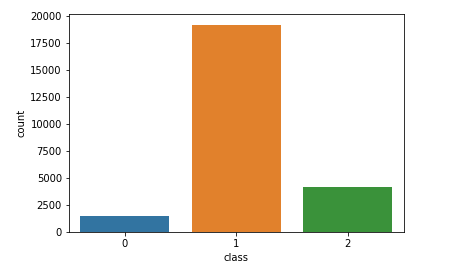
\includegraphics[width=1.1\linewidth, height=0.25\textheight]{pictures/HistOfData}
	\caption[Histogram showing number of labeled classes]{Histogram shows the imbalanced dataset. Tweets from dataset were extracted using \textit{hate} words from Hatebase but not many of them contained hate speech.}
	\label{fig:histofdata}
\end{figure}

We use the dataset annotated by CrowdFlower workers. The workers were asked to annotate 25000 tweets into 3 categories: hate speech (class 0), offensive language (class 1) and speech that contains neither hate speech nor offensive language (class 2). A clear imbalance in the dataset is shown in a histogram displayed in Figure \ref{fig:histofdata}.\cite{Davidson2017AutomatedHS}, creators of the used dataset, used logistic regression to detect hate speech. Even though their model was rather successful, they still struggled with separating hate speech from offensive language. In this paper, we explore the use of active learning to deal with the problems of separating offensive language from hate speech and solving the imbalance of the used dataset.


\section{Related work}

Hate speech today is one big unresolved problem. Even companies like Facebook are still struggling with it. It is important to separate hate speech from offensive language, even so because of new laws against hate speech\cite{Davidson2017AutomatedHS}. As said in \cite{Davidson2017AutomatedHS} offensive language is mostly used in everyday life and often doesn't do any harm. Author in that same paper tried few variants of models and decided that Logistic Regression with L2 regularization is best model right now.
While this i problem yet to be solved there is no much features that surely works. In \cite{Davidson2017AutomatedHS} they used several features to capture information about syntactic and semantic structures. Porter stammer is used to create unigram, bigram and trigram features and then used TF-IDF to put weights to them. Using NLTK they constructed Part of Speech tags as features. They showed that their model is working great, and got pretty high official metrics (precision, recall and F1 score). In introduction of their paper they stated that lexical structures often mislead model and produces false positives on hate speech.
In \cite{WaseemUnderstandingAbuse} authors stated and gave example of one reason why today we can't get relevant scores or dataset. As stated problem is that there is no consensus on what falls under what category. So they proposed new separation methods. It is contained out of two questions:
\begin{itemize}
	\item \textit{Is the language directed towards a specific individual or entity or is it directed towards a generalized group?}
	\item \textit{Is the abusive content explicit or implicit?}
\end{itemize}
Answering those questions we can differ four main classes:
\begin{itemize}
	\item \textit{Directed Implicit}
	\item \textit{Generalized Implicit}
	\item \textit{Directed Explicit}
	\item \textit{Generalized Explicit}
\end{itemize}
\\\cite{ChenSVMFeatures} shows that one can implement feature selection methods into SVM it self. This could possibly make great future work in trying to achieve end-to-end solution for hate speech identification problem, as we encountered problem of high number of features, and high CPU and RAM requirement as result of that. In our paper we used baseline features because we didn't want to focus our selves on feature selection. Given approach in \cite{ChenSVMFeatures} gives us idea how to improve our model later on.
\\Problem of data size and time needed to manually label same data was always been in machine learning. That's why active learning as semi-supervised approach is developed. \cite{LuoALPlankton} proposed new active learning model based on multi-class support vector machines. They showed that there is a way to make SVM work with probabilities and give us proper active learning model. Even though we didn't implement this model, plan is to implement it in the future and test it on state-of-the-art models. Their algorithm works as follows:
\begin{itemize}
	\item 1. Start with an initial training set and an unclassified set.
	\item 2. A multi-class support vector machine is built using the current training set.
	\item 3. Compute the probabilistic outputs of the classification results for each data on the unclassified set. Suppose the class with highest probability is a and the class with second highest probability is b. Record the value of P(a) and P(b) for each unclassified data.
	\item 4. Remove the data from the unclassified set that have the smallest difference in probabilities between them (P(a) − P(b)) for the two highest probability classes, obtain the correct label from human experts and add the labeled data to the current training set.
	\item 5. Go to 2
\end{itemize}
5\\In \cite{YangMultiClassAL} authors introduced their own active learning model based on multi-class SVMs. It is little different from one before on manner that they calculate probability on each data in unlabeled pool. Given that model is computational expensive if unlabeled pool in large size. Their experiment also show that they outperform state-of-the-art models, which can only be a sign to continue further on out work to get end-to-end solution for hate speech identification.
\section{Preparing data}
We used dataset that was introduced in \cite{Davidson2017AutomatedHS}. They prepared the data by annotating the twitter posts with three available classes, 0 meaning it's a hate speech, 1 being an offensive language and 2 being nothing of previous two. People from CrowdFlower annotated the data by marking each tweet, they classified the tweet by majority class. Minimum of annotators for each tweet was three.
As seen in Figure\ref{fig:histofdata} data is unevenly distributed. That has big influence on learning outcomes. Data preparation was in given order.
\\First we had to clear the text from all of the usual twitter stuff. Stuff like hash tag or @. Writing regular expression to automate this was a way to go. Except hash tags and special signs we also removed URL, dates, times, etc.
\\After cleaning text same text is switched to lower case and got tokenized. Text was stemmed using Porter stammer.
\\Using \textit{NLTK} library we removed all classical stop words in English language. After tokenization 50 most frequent words are removed, that allowed us to lower size of our features. That same size was one of the biggest problems in our work.
We tried doing that on our baselines and got much better results so we used that approach with active learning.
\\The last thing we had to do is to turn this tokens to vectors.We used TF-IDF vectorizer, from \textit{sklearn} library, to extract features from our text. After this preparations we where ready to train our baseline models and our active learning method.
\begin{table*}[!t]
	\centering
	\resizebox{\textwidth}{!}{%
		\begin{tabular}{lll}
			&                       &                                                                                                                             \\ \hline
			\multicolumn{1}{|l|}{Tweets before cleaning} & \multicolumn{1}{l|}{} & \multicolumn{1}{l|}{Lmao RT @MoeMartin44 The in soles in Reebok Classics can't even handle diabetic weight Rick Ross holds} \\ \hline
			\multicolumn{1}{|c|}{Array of words}         & \multicolumn{1}{l|}{} & \multicolumn{1}{l|}{lmao, sole, reebok, classic, can't,  even, handl,  diabet, weight, rick,  ross, hold}                   \\ \hline
		\end{tabular}%
	}
	\caption{First row shows the original tweet post from dataset, the second row shows cleaned, tokenized and steammed tweet post}
	\label{tbl:prepData}
\end{table*}

\\Table \ref{tbl:prepData} shows the output of our data preparation. After cleaning, tokenization, etc. we got array of words that represents input post in dataset.

\section{Model}
As stated above problem with machine learning is that we need a lot of data to train model properly. Hate speech identification problem is that there is no relevant and good enough database. Database introduced in \cite{Davidson2017AutomatedHS} has lack of equal distribution of data across all classes. To sidestep that problem we decided to go with semi-supervised model. So called active learning.
\\While this is just a brief overview and some kind of prototype to show us if active learning is good approach, we introduced just one of the baseline models for active learning. Label Spreading and Label Propagation are only two semi-supervised model that one can find in \textit{sklearn} library.
\\In \cite{LuoALPlankton} and \cite{YangMultiClassAL} it is shown that active learning can be of much use when coming to problem of to few data.
\\Idea of active learning is that in first step we take small subset out of training set, and train our model on it. In next steps we need to calculate probabilities of good estimation of model. Given these probabilities we then choose subset of that data that has the lowest probability of estimation. After that model is trained once again. This continues until maximum number of iteration is reached, metrics are satisfying, or model reached some other condition.
\\In our work we used $100$ iterations, and lowest $100$ probabilities. These number were chosen because, when tried greater number of new data in training set we would lose precision in calculating how much data we need to have the results satisfying. With these numbers we get desired results after half of iterations, and we kept running other half too see how will model behave.

\begin{table*}[b]
	\centering
	\caption{Metric evolving through iterations}
	\label{tbl:metrics}
	\begin{tabular}{|lllllllllll|l|l|}
		\hline
		& Iteration             & \multicolumn{3}{c}{0}                                                             &                       & \multicolumn{3}{c}{60}                                                            &                       & \multicolumn{3}{c|}{100} \\ \hline
		\multicolumn{1}{|l|}{}  & \multicolumn{1}{l|}{} & \multicolumn{1}{l|}{P}    & \multicolumn{1}{l|}{R}    & \multicolumn{1}{l|}{F1}   & \multicolumn{1}{l|}{} & \multicolumn{1}{l|}{P}    & \multicolumn{1}{l|}{R}    & \multicolumn{1}{l|}{F1}   & \multicolumn{1}{l|}{} & P      & R      & F1     \\ \hline
		\multicolumn{1}{|l|}{0} & \multicolumn{1}{l|}{} & \multicolumn{1}{l|}{0.11} & \multicolumn{1}{l|}{0.04} & \multicolumn{1}{l|}{0.06} & \multicolumn{1}{l|}{} & \multicolumn{1}{l|}{0.35} & \multicolumn{1}{l|}{0.20} & \multicolumn{1}{l|}{0.25} & \multicolumn{1}{l|}{} & 0.37   & 0.19   & 0.25   \\ \hline
		\multicolumn{1}{|l|}{1} & \multicolumn{1}{l|}{} & \multicolumn{1}{l|}{0.80} & \multicolumn{1}{l|}{0.91} & \multicolumn{1}{l|}{0.85} & \multicolumn{1}{l|}{} & \multicolumn{1}{l|}{0.82} & \multicolumn{1}{l|}{0.91} & \multicolumn{1}{l|}{0.86} & \multicolumn{1}{l|}{} & 0.82   & 0.91   & 0.86   \\ \hline
		\multicolumn{1}{|l|}{2} & \multicolumn{1}{l|}{} & \multicolumn{1}{l|}{0.47} & \multicolumn{1}{l|}{0.30} & \multicolumn{1}{l|}{0.37} & \multicolumn{1}{l|}{} & \multicolumn{1}{l|}{0.53} & \multicolumn{1}{l|}{0.36} & \multicolumn{1}{l|}{0.43} & \multicolumn{1}{l|}{} & 0.51   & 0.36   & 0.42   \\ \hline
	\end{tabular}
\end{table*}

\\Table \ref{tbl:metrics} show how are metric improved through time. In table \ref{tbl:metrics} we can see that optimal, and peak of model is on $60$ iterations. That's about $6000$ labeled data on which we train our model.

\\Active learning algorithm goes like this:
\begin{itemize}
	\item \textit{1. Select m size subset from training set}
	\item \textit{2. Train label spreading model on given subset}
	\item \textit{3. Predict probabilities on remaining set from training set}
	\item \textit{4. Select n worst probabilities and put that data expand initial training set with these data}
	\item \textit{5. Go to 2.}
\end{itemize}


\bibliographystyle{tar2018}
\bibliography{tar2018} 

\end{document}

